% !TEX root = ../thesis-example.tex
%
\chapter*{Introduction Générale}
\label{sec:intro}
\addcontentsline{toc}{chapter}{\nameref{sec:intro}}

\section{Contexte et Motivations}
\label{sec:intro:contexte}
Une décision judiciaire peut être définie soit comme  le résultat rendu par des juges à l'issue d'un procès, ou bien un document décrivant une affaire judiciaire en résumant les faits, les procédures suivies, la solution des juges, et les raisons qui les y ont conduits. %Nous considérons le nom "résultat" pour la première définition, et pour la seconde, "décision jurisprudentielle", "décision judiciaire", "décision de justice" ou simplement  "décision".
Les décisions judiciaires sont essentielles pour les juristes parce qu'elles sont des sources d'interprétation de la loi.
Ce mémoire présente les résultats d'une étude visant à automatiser l'extraction d'information à partir de ces documents afin de faciliter la recherche et les analyses descriptives et prédictives d'un corpus jurisprudentiel. Ces analyses sont indispensables pour les pratiquants du droit car elles fournissent un ensemble important d'information  nécessaires pour diverses études.  Les avocats ont par exemple l'habitude de rechercher et d'analyser les décisions afin de résoudre les problèmes en cours ouvvv conseiller leurs clients.  La question à la base de notre étude est celle de savoir "Comment exploiter un corpus de décisions pour analyser, voire prédire, les décisions des juges sachant que l'interprétation subjective des règles juridiques rend l'application de la loi non déterministe ?" Cette question intéresse de nombreuses entreprises telles que LexisNexis avec son système LexMachina\footnote{https://lexmachina.com}, et de jeunes startups françaises telles que Predictice\footnote{http://predictice.com} et CASE LAW ANALYTICS\footnote{http://caselawanalytics.com}. Afin d'y répondre, nous sommes partis d'une conception théorique considérant la demande des parties ou prétention comme le concept central d'une décision (Figure \ref{fig:intro:demande-central}) et tout autour s'affectent d'autres concepts, notamment, le résultat des juges relatif à cette prétention, le fondement juridique de la prétention ou norme, la catégorisation des prétentions, et ensuite les différentes circonstances factuelles dans lesquelles cette prétention est généralement formulée.vvvv En fait, La granularité de l'analyse est affinée jusqu'à la demande car dans une décision, les juges apportent une réponse à chaque demande, et par conséquent une partie peut voir certaines de ses demandes acceptées complètement, lorsque d'autres accordées partiellement, et le reste est rejetée. Ceci est revoit en effet les modélisations prédictives qui ne s'attardaient qu'à déterminer globalement si le plaintif a  gagné ou perdu le procès sans estimer précisement ce que chaque partie a obtenu. Par ailleurs, les juristes s'intéressent généralement à un type de contentieux à la fois et surtout à des types particuliers de demandes s'appuyant sur une règle ou un principe juridique appelé "fondement". Ainsi, une analyse devrait se faire dans un contexte bien précis, défini par ces différents concepts.

\begin{figure}[h!]
    \centering
    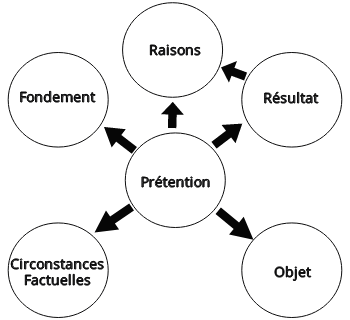
\includegraphics[scale=0.75]{demande-central.png}
    \caption{La demande est centrale aux concepts liés à l'analyse des décisions}
    \label{fig:intro:demande-central}
\end{figure}




\section{Enoncé des problèmes}
\label{sec:intro:probleme}
L'analyse automatique de décisions jurisprudentielles fait références à de nombreux problèmes rencontrés par les juriste lors de leur analyse manuelle (\textcolor{red}{par exemple?}). Dans le cadre de notre travail, nous avons définies et traités les quelques problèmes principaux décrits dans les sous-sections suivantes.
\subsection{Sectionnement des documents}
Le sectionnement des décisions de justice est important pour donner une première structure grossière aux documents. Cette structuration pourrait faciliter tout autant la lecture manuelle des documents par la localisation plus rapide des informations, et l'organisation des tâches d'extraction automatique d'information. Notre principale contribution lors du traitement de ce problème a été de réaliser une étude comparative de modèles d'étiquetage de séquence, bien établis au sein de la communauté de traitement automatique du langage naturel (TALN),  pour la reconnaissance de sections prédéfinies. 

\subsection{Annotation de métadonnées}

\subsection{Identification de données relatives aux demandes}

\subsection{Identification des circonstances factuelles}

\section{Méthodologie}
\label{sec:intro:methodologie}


\section{Résultats}
\label{sec:intro:résultats}

\section{Structure du mémoire}
\label{sec:intro:organisation}

\textbf{Chapitre \ref{sec:literature}} \\[0.2em]
%blindtext

\textbf{Chapitre \ref{sec:structuration}} \\[0.2em]
%\blindtext

\textbf{Chapitre \ref{sec:quanta}} \\[0.2em]
%\blindtext

\textbf{Chapitre \ref{sec:sensresultat}} \\[0.2em]
%\blindtext

\textbf{Chapitre \ref{sec:similarite}} \\[0.2em]
%\blindtext

\textbf{Chapitre \ref{sec:conclusion}} \\[0.2em]

\textbf{Les annexes \ref{sec:demo}} \\[0.2em]
